\section{Tautologi, Kontradiksi, dan Kontingensi}

\textbf{Tautologi} adalah proposisi yang selalu bernilai benar untuk setiap interpretasi variabel proposisional \cite{rosen2019,stanford_intrologic}. Contoh klasik tautologi adalah $p \vee \neg p$ (hukum excluded middle): baik $p$ benar maupun $p$ salah, ekspresi tersebut tetap benar. Tautologi memainkan peran penting dalam logika karena argumen yang valid dapat direpresentasikan sebagai implikasi yang tautologis: premis-premis mengimplikasikan kesimpulan sehingga implikasi tersebut selalu benar \cite{forallx}.

\textbf{Kontradiksi} adalah proposisi yang selalu bernilai salah untuk setiap interpretasi \cite{rosen2019,stanford_intrologic}. Contoh: $p \wedge \neg p$, yang menyatakan bahwa $p$ sekaligus tidak $p$---suatu hal yang mustahil. Kontradiksi berguna dalam pembuktian dengan reductio ad absurdum: jika dari suatu asumsi kita sampai pada kontradiksi, maka asumsi tersebut salah dan kita dapat menyimpulkan negasinya \cite{stanford_intrologic}.

\textbf{Kontingensi} adalah proposisi yang kadang benar dan kadang salah, bergantung pada interpretasi variabelnya \cite{levin_discrete,stanford_intrologic}. Contohnya $p \wedge q$: benar bila $p$ dan $q$ keduanya benar, salah untuk kombinasi lain. Sebagian besar proposisi sehari-hari bersifat kontingen; hanya proposisi dengan struktur khusus (misalnya hukum excluded middle) yang menjadi tautologi atau kontradiksi \cite{stanford_intrologic}.

Hubungan penting antara ekuivalensi dan tautologi: dua proposisi $P$ dan $Q$ ekuivalen secara logika ($P \equiv Q$) jika dan hanya jika $P \leftrightarrow Q$ merupakan tautologi \cite{rosen2019,forallx}. Artinya, untuk membuktikan ekuivalensi kita dapat menunjukkan bahwa biconditional-nya selalu benar. Metode ini sering lebih praktis daripada membandingkan tabel kebenaran $P$ dan $Q$ secara terpisah.

Tabel~\ref{tab:contoh-tautologi-kontradiksi} memberi contoh formula untuk setiap jenis beserta nilai di semua interpretasi \cite{rosen2019,stanford_intrologic}.

\begin{table}[htbp]
\centering
\small
\begin{tabular}{|l|>{\raggedright\arraybackslash}p{4.5cm}|l|}
\hline
\textbf{Jenis} & \textbf{Contoh formula} & \textbf{Nilai di semua interpretasi} \\
\hline
Tautologi & $p \vee \neg p$, \ $p \rightarrow p$, \ $(p \rightarrow q) \leftrightarrow (\neg p \vee q)$ & Selalu B \\
\hline
Kontradiksi & $p \wedge \neg p$ & Selalu S \\
\hline
Kontingensi & $p \wedge q$, \ $p \rightarrow q$, \ $p \vee q$ & Tergantung (ada B dan S) \\
\hline
\end{tabular}
\caption{Contoh tautologi, kontradiksi, dan kontingensi}
\label{tab:contoh-tautologi-kontradiksi}
\end{table}

Untuk $n$ variabel proposisional, tabel kebenaran memiliki $2^n$ baris. Grafik pada Gambar~\ref{fig:baris-tabel-bab4} menunjukkan pertumbuhan eksponensial ini; memeriksa ``semua interpretasi'' berarti mengevaluasi formula pada $2^n$ kombinasi nilai kebenaran \cite{levin_discrete}.

\begin{figure}[htbp]
\centering
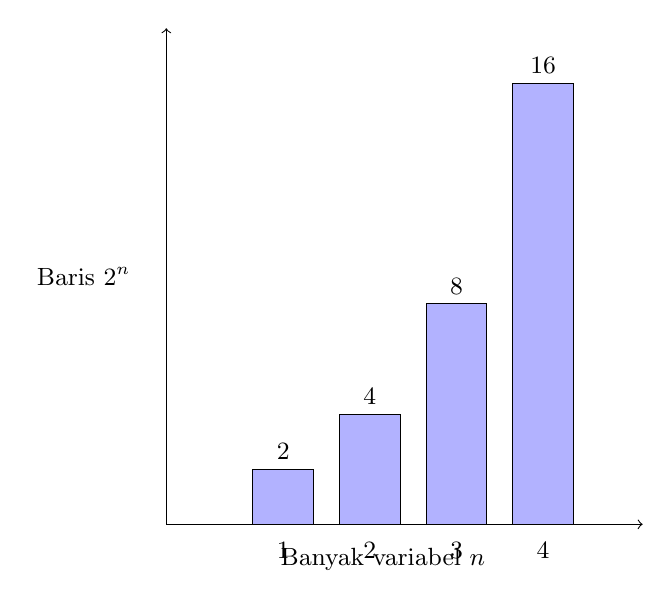
\begin{tikzpicture}[y=0.35cm, x=1.1cm, font=\small]
  \draw[->] (0,0) -- (0,18);
  \draw[->] (0,0) -- (5.5,0);
  \node[below] at (2.5,-0.5) {Banyak variabel $n$};
  \node[left] at (-0.3,9) {Baris $2^n$};
  \foreach \n/\v in {1/2, 2/4, 3/8, 4/16} {
    \draw[fill=blue!30] (\n,0) rectangle (\n+0.7,\v);
    \node[below] at (\n+0.35,-0.3) {\n};
    \node[above] at (\n+0.35,\v) {\v};
  }
\end{tikzpicture}
\caption{Banyak baris tabel kebenaran: $2^n$ untuk $n$ variabel proposisional}
\label{fig:baris-tabel-bab4}
\end{figure}

\begin{contoh}
\textbf{Tabel kebenaran singkat untuk tautologi dan kontradiksi}

Untuk satu variabel $p$:
\begin{center}
\small
\begin{tabular}{|c|c|c|}
\hline
$p$ & $p \vee \neg p$ (tautologi) & $p \wedge \neg p$ (kontradiksi) \\
\hline
B & B & S \\
S & B & S \\
\hline
\end{tabular}
\end{center}
Kolom $p \vee \neg p$ selalu B; kolom $p \wedge \neg p$ selalu S.
\end{contoh}

Fungsi Python berikut mengklasifikasikan formula (diberikan sebagai fungsi evaluasi) ke dalam tautologi, kontradiksi, atau kontingensi \cite{python_docs_boolean,levin_discrete}.

\begin{contoh}
\textbf{Mengidentifikasi tautologi, kontradiksi, dan kontingensi dengan Python}

\begin{lstlisting}[style=pythonstyle, caption={Fungsi is\_tautology, is\_contradiction, is\_contingency untuk dua variabel}]
from itertools import product

def is_tautology(formula_fn):
    """Cek apakah formula selalu True untuk semua (p, q)."""
    return all(formula_fn(p, q) for p, q in product([True, False], repeat=2))

def is_contradiction(formula_fn):
    """Cek apakah formula selalu False untuk semua (p, q)."""
    return all(not formula_fn(p, q) for p, q in product([True, False], repeat=2))

def is_contingency(formula_fn):
    """Cek apakah formula kadang True dan kadang False."""
    vals = [formula_fn(p, q) for p, q in product([True, False], repeat=2)]
    return True in vals and False in vals

# Contoh: p or not p (tautologi), p and not p (kontradiksi), p and q (kontingensi)
taut = lambda p, q: p or (not p)
contra = lambda p, q: p and (not p)
contig = lambda p, q: p and q

print("p or ~p tautologi?", is_tautology(taut))       # True
print("p and ~p kontradiksi?", is_contradiction(contra))  # True
print("p and q kontingensi?", is_contingency(contig))  # True
\end{lstlisting}
\end{contoh}

Dalam informatika, pemahaman tautologi, kontradiksi, dan kontingensi diterapkan pada verifikasi perangkat lunak, optimisasi kondisi Boolean dalam program, dan SAT solving \cite{levin_discrete,rosen2019}. Ekspresi yang tautologis dapat dioptimalkan atau disederhanakan; kondisi yang kontradiksi menandakan bug (dead code); sedangkan kondisi kontingen perlu dievaluasi pada runtime. Pengenalan pola proposisi membantu programmer menulis kode yang lebih efisien dan mudah dipelihara.

\begin{itemize}
  \item \textbf{Tautologi}: Proposisi yang selalu benar untuk semua interpretasi. Contoh: $p \vee \neg p$.
  \item \textbf{Kontradiksi}: Proposisi yang selalu salah. Contoh: $p \wedge \neg p$.
  \item \textbf{Kontingensi}: Proposisi yang kadang benar dan kadang salah.
\end{itemize}
